\subsection{Customer Details Page}
\bigskip
\paragraph{}
In Customer Details page, there is a table that contains all the registered customers' detailed information like phone numbers and addresses. Website admins can see and modify the customers information, add new customer or delete an existing one. Select one customer from the table and then click Edit button, admins can edit that customer's information. Or by clicking the Delete button, admin can delete one existing customer from website and also from the database. On the other hand, if admin want to add new customer to the system, he/she click the Add button and add customer. 
\bigskip
\bigskip
\bigskip
\begin{figure}[h]
\centerline{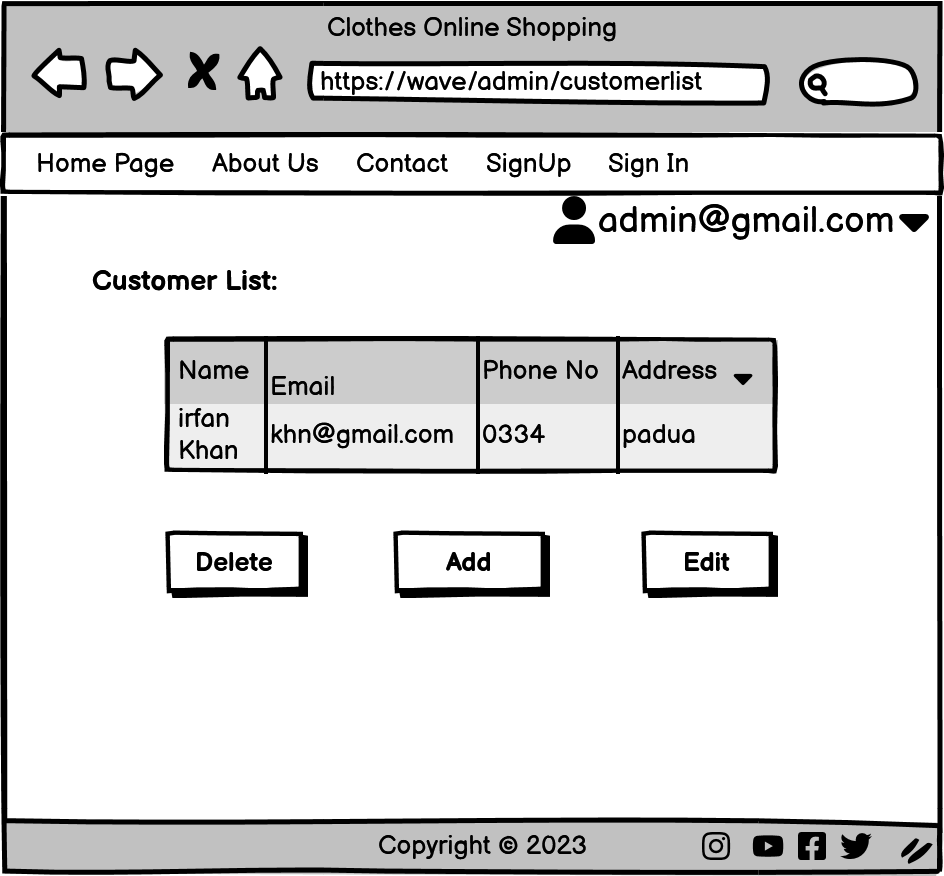
\includegraphics[scale=1.]{images/Customer Details.png}}
\caption{Customer Details Page}
\label{fig}
\end{figure}

\newpage
\subsection{Add Customer Page}
\bigskip
\paragraph{}
In Add Customer page, admin will fill manually the required fields; name, e-mail, password, phone number and address, and then, click the Add button at the end of the page. By clicking the Add button, new customer is created and added to the system and database. A notification e-mail will be sent to the customer's e-mail address. 
\bigskip
\bigskip
\bigskip
\begin{figure}[h]
\centerline{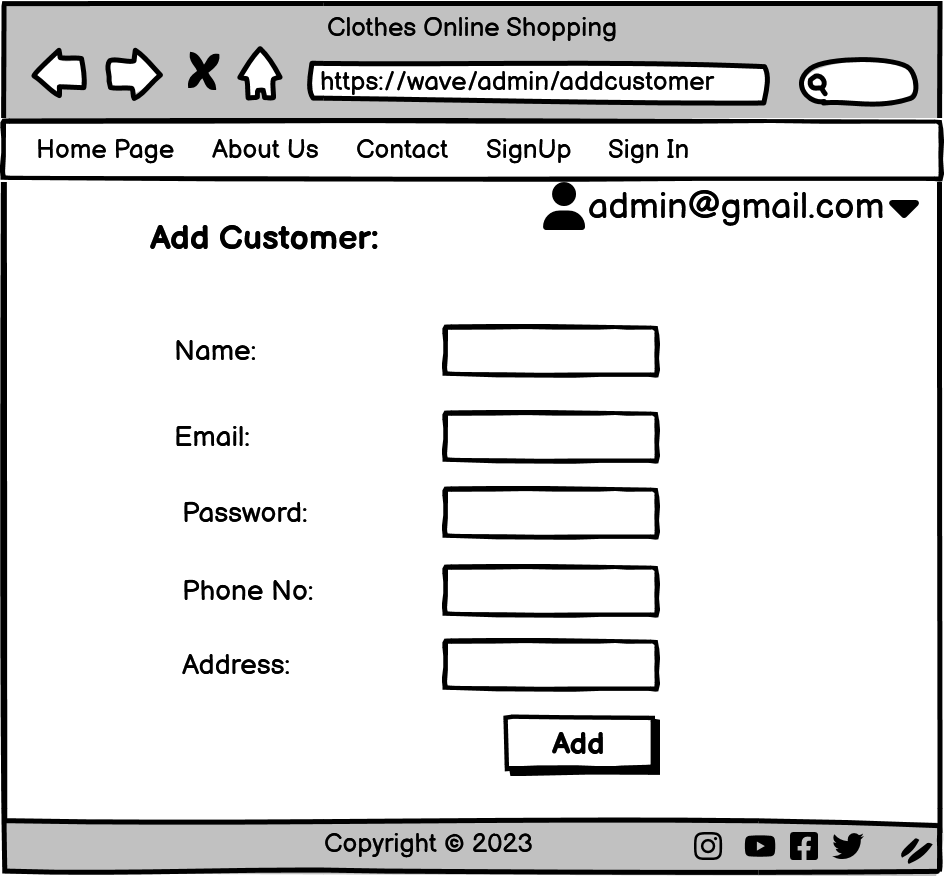
\includegraphics[scale=1.]{images/Add Customer.png}}
\caption{Add Customer Page}
\label{fig}
\end{figure}

\newpage
\subsection{Edit Customer Page}
\bigskip
\paragraph{}
In Edit Customer page, admins can see detailed customer information and change them. After changing the fields, they click the Edit button and submit the changes to the database. A notification e-mail related with the changes will be sent to the customer's e-mail address.  

\bigskip
\bigskip
\bigskip
\begin{figure}[h]
\centerline{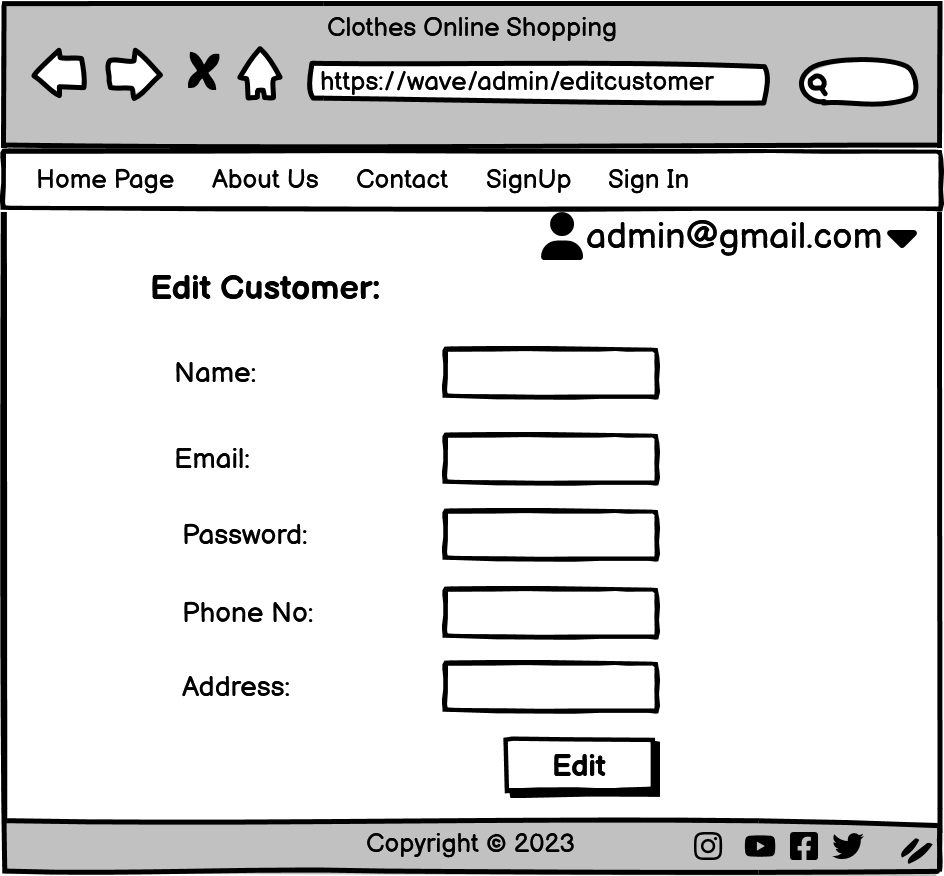
\includegraphics[scale=1.]{images/Edit Customer.png}}
\caption{Edit Customer Page}
\label{fig}
\end{figure}